\section[Processes Involve a New Person]{Processes Involve a Person New to the Process\label{sec:new-person}\iftoggle{shortsectiontitle}{\sectionmark{Processes Involve a New Person}}{}}
\iftoggle{shortsectiontitle}{\sectionmark{Processes Involve a New Person}}{}

% LONG1 shows up in the TOC
% LONG2 is the section title

% https://graphthinking.blogspot.com/2022/07/bureaucratic-processes-typically.html

% The IPYNB notebook is in
% https://drive.google.com/drive/u/0/folders/1awZYk4EisFIR3mY1iF2X7Hb6CwcNDavp

Bureaucratic processes require working with other people. One source of friction is that participants may lack familiarity with the process. 

This observation can be quantified with a small number of assumptions. 
When there are more inexperienced people than experienced people, 
the distribution of team membership tenure might fit a \href{https://en.wikipedia.org/wiki/Power_law}{power law distribution}.
\index{Wikipedia!power law@\href{https://en.wikipedia.org/wiki/Power_law}{power law}}
%\footnote{See \href{https://numpy.org/doc/stable/reference/random/generated/numpy.random.power.html}{numpy.random.power} documented on https://numpy.org/doc.}
What matters in this context is how long the team member has been in their role rather than how long they've been a member of the organization. Assume a max tenure of ten years~\cite{2022_BLS_tenure}. With these conditions, if the process involves five people then the least experienced member will have a median of 100 calendar days of experience.

% image float options:
% https://tex.stackexchange.com/a/32605/235813
\begin{figure}[!htb] %[H]
    \centering % 0.8 is too small
    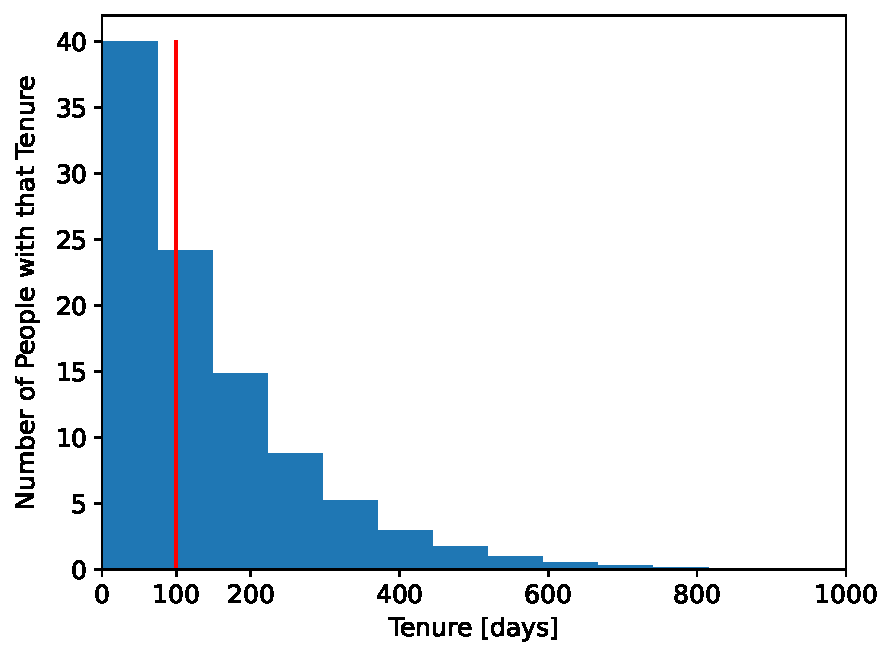
\includegraphics[width=1\textwidth]{images/tenure_power_distribution_a5_with_max_tenure10_and_5_participants.pdf}
    \caption{For a population of 100 peole, the power law distribution of tenure using the \href{https://en.wikipedia.org/wiki/Probability_density_function}{probability density function}
    \index{Wikipedia!probability density function@\string\href{https://en.wikipedia.org/wiki/Probability_density_function}{probability density function}}
    described by $a\ x^{(a-1)}$ where the free parameter $a=5$. The median tenure of the youngest participant  in a process with five people is 100 days, indicated by the horizontal line. }
    \label{fig:tenure-powerlaw-5-participants-tenure10}
\end{figure}


Three calendar months (or 70 business days) may be inadequate for complex processes or processes that are infrequent (quarterly or annual), especially if there was no training. When the number of participants is ten people, then the median tenure of the youngest participant is 51 calendar days (37 business days).

\ \\

\begin{samepage}
To recap, the assumptions made were:
\begin{itemize}
    \item Random, independent sampling of organization members. 
    \item Tenure in your role matters, not the tenure in the organization. (This assumption excludes transfer learning among roles.)
    \item Tenure in role fits a power law distribution.
    \item The power law distribution is characterized by (free parameter $a=5$, max tenure=10 years). 
    \item There are five people involved in the process.
\end{itemize}
\end{samepage}
If that last parameter is varied, the estimate of three months as the median  is reasonable for processes with five or more participants.

% image float options:
% https://tex.stackexchange.com/a/32605/235813
\begin{figure}[!htb]  %[H]
    \centering % 0.8 is too small
    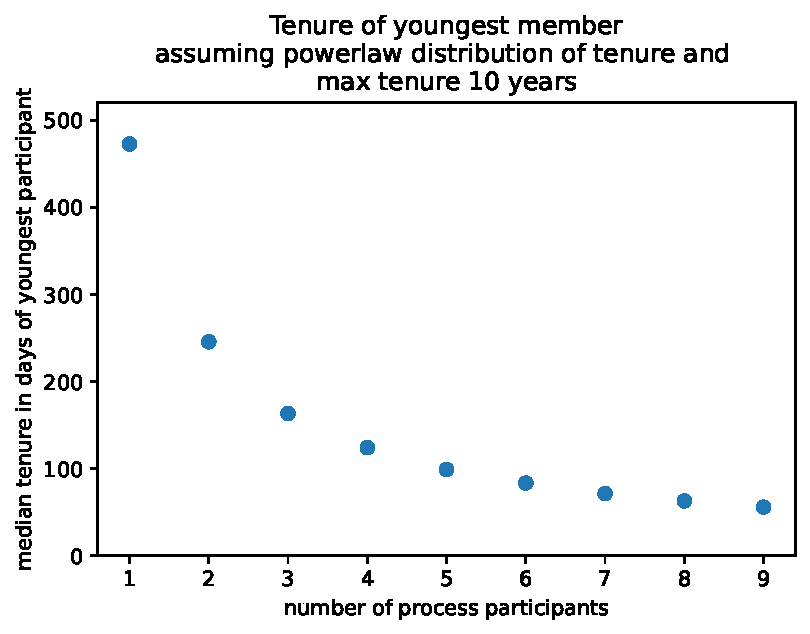
\includegraphics[width=1\textwidth]{images/tenure_power_distribution_a5_with_max_tenure10.pdf}
    \caption{Median tenure of the youngest participant (in calendar days) as a function of the number of process participants with tenure following a 
    \href{https://en.wikipedia.org/wiki/Probability_density_function}{probability density function},
    \index{Wikipedia!probability density function@\string\href{https://en.wikipedia.org/wiki/Probability_density_function}{probability density function}}
    $a=5$, and max tenure of ten years.}
    \label{fig:tenure-powerlaw-5-participants}
\end{figure}


Even when there's a single participant, the median tenure is less than two years because of the power law distribution of tenure.

% Uniform Distribution of Tenure instead of a Power Law Distribution
What if the power law distribution of tenure were replaced with a uniform distribution?
Surprisingly the shape of the distribution of the youngest participant's tenure is not uniform, see Figure~\ref{fig:tenure-uniform-5-participants}. The median tenure of the youngest member of a process with five participants is 15 months. 

% image float options:
% https://tex.stackexchange.com/a/32605/235813
\begin{figure}[!htb]  %[H]
    \centering
    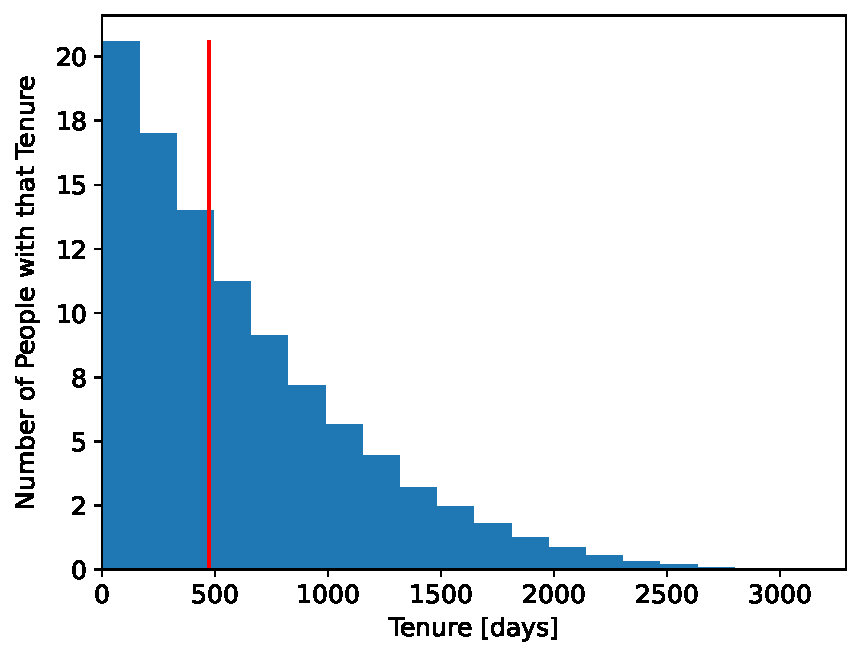
\includegraphics[width=1\textwidth]{images/tenure_uniform_distribution_with_max_tenure10_and_5_participants_median472.pdf}
    \caption{The median tenure of the youngest participant
 in a process with five people is 472 days when the distribution of tenure is uniform. The population size has been normalized to 100 people.}
    \label{fig:tenure-uniform-5-participants}
\end{figure}



% https://latex.org/forum/viewtopic.php?t=17111
\FloatBarrier